
\chapter{Architecture Assumptions}
Since memory disaggregation architecture is an open research topic, we make the following architecture assumptions.
We assume a partial disaggregation model where each compute node has a small amount of local memory. Access to this local memory will not incur any extra delay. Rest of the memory is located on remote memory "blade" located anywhere across the data center. The granularity of the remote memory is in pages of size 4kB which is default page size in Linux. A remote memory is requested though standard hardware protocol whenever compute node needs to access remote memory. High speed network interconnection is used to setup communication between devices.  A local page is evicted based on the eviction policy. Then the requested remote page is transferred over the network to local memory, incurring a network delay. Figure \ref{fig:arch} shows a high level memory flow when remote memory is accessed.

We assume that the same memory is not shared across multiple compute nodes at the same time, so there will not be local memory coherency issue to be handled. We do not consider queuing delays over the interconnect since there is not enough literature about the type of networking technologies that will be used and the interconnect network architecture.

\begin{figure}[tbp]
	\centering
%	\includesvg{assumption/architecture}
	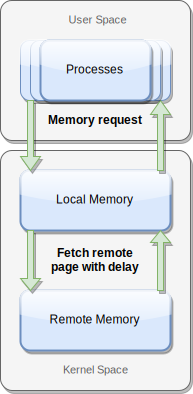
\includegraphics{assumption/architecture.pdf}
	\caption[Disaggregated Memory Flow]{Disaggregated memory flow.}
	\label{fig:arch} 
\end{figure}


%%% Local Variables: 
%%% mode: latex
%%% TeX-master: "../mainrep"
%%% End: 
